% SPDX-FileCopyrightText: 2026 Cyprien PIERRE
% SPDX-License-Identifier: CC-BY-4.0
\documentclass[tikz,border=5pt]{standalone}
\usepackage[T1]{fontenc}
\usepackage{lmodern}
\usetikzlibrary{arrows.meta,positioning}
\begin{document}
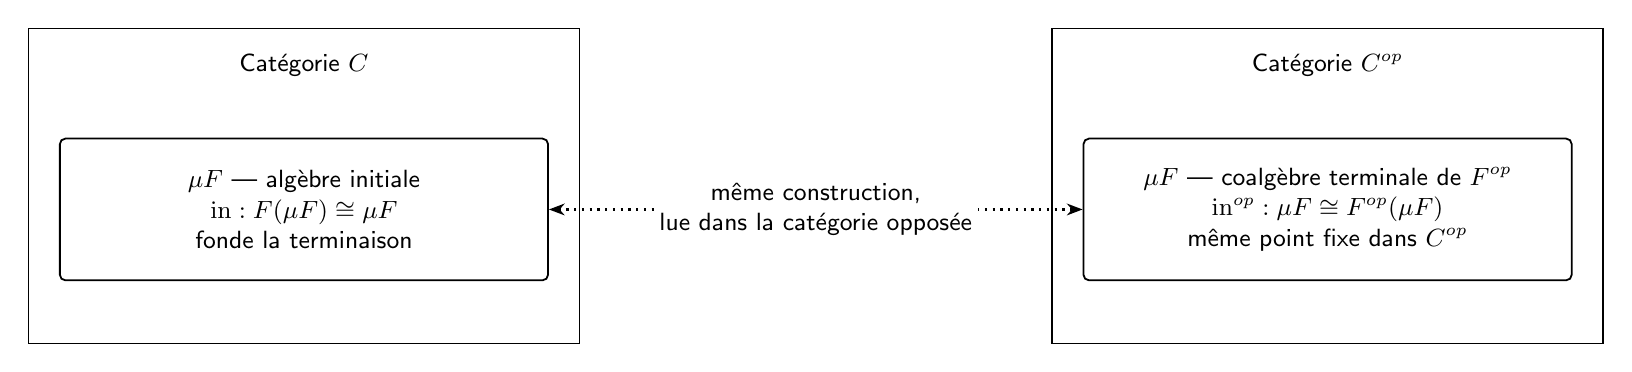
\begin{tikzpicture}[
  font=\sffamily\small,
  frame/.style={draw, line width=.5pt},
  box/.style={draw, rounded corners=2pt, align=center, line width=.65pt, minimum height=18mm, minimum width=62mm},
  link/.style={{Stealth[length=2mm]}-{Stealth[length=2mm]}, dotted, line width=.8pt}
]
\draw[frame] (0,0) rectangle (70mm,40mm);
\node[anchor=north] at (35mm,38mm) {Catégorie $C$};
\node[box] (mu) at (35mm,17mm) {$\mu F$ --- algèbre initiale\\$\mathrm{in} : F(\mu F) \cong \mu F$\\fonde la terminaison};
\draw[frame] (130mm,0) rectangle (200mm,40mm);
\node[anchor=north] at (165mm,38mm) {Catégorie $C^{op}$};
\node[box] (nu) at (165mm,17mm) {$\mu F$ --- coalgèbre terminale de $F^{op}$\\$\mathrm{in}^{op} : \mu F \cong F^{op}(\mu F)$\\même point fixe dans $C^{op}$};
\draw[link] (mu) -- node[fill=white, align=center, inner sep=2pt] {même construction,\\lue dans la catégorie opposée} (nu);
\end{tikzpicture}
\end{document}
